\documentclass[12pt,a4paper, german,oneside, headinclude, headsepline,plainheadsepline,BCOR20mm, DIV18,parskip=half, openright, numbers=noenddot, captions=tableheading,version=first,listof=totoc,version=first]{scrbook}

\hfuzz=20pt
\vfuzz=20pt

%--------------- Packages ----------------
\usepackage[ngerman]{babel}
\usepackage[utf8]{inputenc}
\usepackage[T1]{fontenc}
\usepackage{lmodern}
\usepackage[centertags]{amsmath} 
\usepackage{tabularx}
\usepackage{graphicx} 
\usepackage{float} 
\usepackage{setspace} 
\usepackage{scrlayer-scrpage}
\usepackage{scrhack}
\usepackage{makeidx}
\usepackage[usenames,dvipsnames,svgnames,table]{xcolor}
\usepackage[absolute]{textpos}
\usepackage{subfigure}
\usepackage{amssymb}
\usepackage{listings}
\usepackage{trfsigns}
\usepackage{siunitx}
\usepackage[abs]{overpic}
\usepackage[colorlinks = false,pdfpagelabels = true,pdfstartview = FitH,bookmarksopen = true,bookmarksnumbered = true,linkcolor = black,plainpages = false,hypertexnames = false,citecolor = black] {hyperref}
\usepackage{pgfplots}
\usepackage[framed,numbered,autolinebreaks,useliterate]{mcode}
\usepackage{xcolor}
\usepackage[
    left = \flqq{},% 
    right = \frqq{},% 
    leftsub = \flq{},% 
    rightsub = \frq{} %
]{dirtytalk}
\lstset{breaklines=true}


\pagestyle{scrheadings}
\renewcommand{\headfont}{\normalfont\sffamily} 
\renewcommand{\pnumfont}{\normalfont\sffamily} 
\ohead[\pagemark]{\pagemark} 
\ifoot[]{}
\ofoot[]{}
\setlength{\headheight}{1.5\baselineskip}
\onehalfspacing

%----------------------- Beginn des Dokuments -----------------------
\begin{document}
\pagenumbering{Roman}
\thispagestyle{empty}
\setcounter{page}{-1}

\includegraphics*[width = \textwidth]{Logos/Logo.pdf}

\vspace{25mm}

{\centering

\LARGE\textbf{{Anleitung}}\\
\vspace{1em}
\large{Für die Multilayout-ESP-Wordclock} \\

\par}


\newpage
\thispagestyle{empty}

\cleardoublepage

\cleardoublestandardpage

\begin{spacing}{1.15}		
\pdfbookmark[1]{Inhaltsverzeichnis}{toc}		
\tableofcontents 		

\end{spacing}

\cleardoublestandardpage

\mainmatter							

\chapter{Einleitung}

Diese Anleitung soll helfen, eine mehrsprachige Wortuhr zu bauen, die auf einem ESP8266 Mikrocontroller und einer programmierbaren LED-Leiste (WS2812 oder SK6812) basiert. Dieses Projekt wurde über mehrere Jahre von einer Vielzahl von Mitwirkenden auf Github entwickelt und frei zur Verfügung gestellt.\\
Eine Wortuhr (auch als Wordclock bekannt) ist ein schönes DIY-Projekt für Anfänger, das Technologie und Design kombiniert, um eine funktionelle und ästhetisch ansprechende Uhr zu schaffen. Egal, ob Sie Anfänger oder erfahrener Bastler sind, dieses Projekt ist eine großartige Gelegenheit, Ihre Fähigkeiten unter Beweis zu stellen und etwas wirklich Besonderes zu schaffen. Die Gestaltungsmöglichkeiten liegen vor allem im Rahmen und in der Wahl der Oberfläche der Uhr. 

\section{Hauptfunktionen}

Die bereitgestellte Software zum Betreiben der Wortuhr hat mehrere Funktionen:

\begin{itemize}
    \item Mehrsprachig (Deutsch, Englisch, Niederländisch, Italienisch, Spanisch, Ungarisch, Französisch, Römänisch, Schweizer Deutsch, Russisch und Schwedisch)
    \item Unterstützung für mehrere Matrizengrößen und LED-Abstände
    \item Farbwechsel der Anzeigefarbe möglich (RGB oder RGBW)
    \item Digitale Uhranzeige
    \item Regenbogenfarbwechsel
    \item Umgebungslicht (als Sekundenzeiger ausgeführt oder Ambientlight)
    \item Automatische Helligkeitsregelung (optional über Sensor)
    \item Offlinebetrieb (optional über entsprechende RTC)
    \item Auswahl an dialektspezifischen Anzeigen
    \item Home-Assistant-Einbindung mit Autodiscovery
\end{itemize}

\section{Uhren Varianten}

\section{Voraussetzungen}

Die folgende Hardware/Software wird für dieses Projekt benötigt:

\subsubsection{Hardware}

\begin{itemize}
    \item NodeMCU oder vergleichbares Board mit einem dem ESP8266 oder ESP8285 Chip
    \item WS2812B RGB-LED-Streifen oder SK6812 RGBW-Streifen
    \item Stromversorgung 5V 2A
    \item Optional: LDR, 10 KOhm-Widerstand
    \item Optional: BH1750 (digitaler Helligkeitssensor, anstallt LDR)
    \item Optional: DS3231 (Echtzeituhr, für den offline Betrieb)
\end{itemize}

\subsubsection{Software}

\begin{itemize}
    \item PlatformIO Core oder IDE (bspw. VIsual Studio Code)
    \item Node.js
    \item Git
\end{itemize}

\chapter{Installation der Wortuhr Software}

\section{Erstmaliges Aufspielen mittels Binary}
Für das erstmalige Aufspielen liegen auf der Githubseite Rechts \say{Releases} zur Verfügung. Dabei handelt es sich um fertig compilierte Versionen der Software. Programme zum aufspielen der binary findet man z.B. unter \say{https://github.com/nodemcu/nodemcu-flasher}

\section{Windows}

\begin{enumerate}
    \item Installieren Sie die aktellsten Versionen von PlatformIO, Node.js und Git manuell
    \item Dadurch wird Visual Studio Code installiert, mit einem PlatformIO-Symbol (Ameisenkopf/Alien) in der Seitenleiste
    \item Gehen Sie zu \say{Quick Access / Miscellaneous} und geben Sie den Befehl \say{Clone Git Project} ein, und geben Sie \href{https://github.com/ESPWortuhr/Multilayout-ESP-Wordclock}{https://github.com/ESPWortuhr/Multilayout-ESP-Wordclock} als URL ein
    \item Gehen Sie dann zu \say{Projekte}, fügen Sie das neue Projekt mit \say{Vorhandenes hinzufügen} zur Liste hinzu und klicken Sie auf \say{Öffnen}.
    \item In der PlatformIO-Seitenleiste erscheint nun \say{Project Tasks}. Wählen Sie den Befehl \say{General / Upload'} (dauert ein paar Minuten, die Software wird zuerst erstellt).
    \item Schließen Sie den ESP8266 über USB an. Wenn die Wortuhr-Software erstellt ist, wird sie auf dem ESP installiert.
\end{enumerate}

\section{MacOS}

Der einfachste Weg wäre mit \say{homebrew}:

\begin{lstlisting}
    brew install platformio
    brew install node
    git clone https://github.com/ESPWortuhr/Wortuhr
    cd Wortuhr
    pio run -t upload
\end{lstlisting}

Dabei ist der ESP8266 über USB angeschlossen. Die Wortuhr-Software wird dabei mittels Plattformio erstellt und auf den ESP übertragen.

\section{Linux}

\begin{lstlisting}
    python3 -c "$(curl -fsSL https://raw.githubusercontent.com/ platformio/platformio/master/scripts/get-platformio.py)"
    sudo apt install npm
    git clone https://github.com/ESPWortuhr/Wortuhr
    cd Wortuhr
    pio run -t upload
\end{lstlisting}

Dabei ist der ESP8266 über USB angeschlossen. Die Wortuhr-Software wird dabei mittels Plattformio erstellt und auf den ESP übertragen.

\section{Update der Firmware über das Web-Frontend}
Mit der Software ist es möglich, die Firmware \textbf{OTA} (over the air), über den in der Uhr eingebauten Webserver zu aktualisieren. Dies ist in den meisten Fällen einfacher als das direkte Flashen.
Ausschlaggebend für diese Vorgehensweise ist, dass die Uhr über WLAN erreichbar ist. Die Update-Schnittstelle ist dann über die Adresse
http://<IP-Adresse der Uhr>:81/update erreichbar (Beispiel: http://192.168.4.1:81/update). Die Adresse der Uhr wird in der Grundeinstellung beim Start als Laufschrift ausgegeben.

\chapter{Hardware}

Für den Aufbau der Wortuhr wird folgende elektronische Hardware benötigt:

\begin{itemize}
    \item NodeMCU oder vergleichbares Board mit ESP8266 oder ESP8285 Chip
    \item RGB-LED-Streifen WS2812B oder RGBW-Streifen SK6812
    \item Stromversorgung 5V 2A
    \item Optional: LDR, 10 KOhm Widerstand
    \item Optional: BH1750 (digitaler Helligkeitssensor, ersetzt LDR)
    \item Optional: DS3231 (Echtzeituhr, für Offline-Betrieb)
\end{itemize}

Ich möchte dich gerne darüber informieren, was du noch alles für den Bau benötigst. Da es verschiedene Arten gibt, eine Uhr zu bauen, werde ich dir hier nur die grundlegenden Dinge aufzählen, die ich oft verwende:

\begin{itemize}
    \item Bilderrahmen (Holz oder Metall mit mindestens 14mm Rahmenhöhe)
    \item Diffusorfolie
    \item Buchstabenmaske
    \item Abstandsgitter (Holz oder Kunststoffschaum)
\end{itemize}

\section{Pegelanpassung}

Der ESP arbeitet intern mit einer Betriebsspannung von 3,3V. Die WS2812(B) Streifen arbeiten dagegen mit 5V. Dies erfordert eine Pegelanpassung, damit die digitalen Signale fehlerfrei zu den Stripes übertragen warden können. Ohne Anpassung kann es auch funktionieren, muss es aber nicht. 
Es gilt: "Der minimale High-Pegel des Ausgangs muss höher sein als der minimale High-Pegel des Eingangs"
Was heißt das im Klartext?
Laut Datenblatt des Stripes sind folgende Pegel notwendig, um ein "sauberes" HIGH und LOW Signal zu bekommen.
Um ein HIGH Signal am Eingang des WS2812B Stripes zu erzeugen, muss laut Datenblatt (Bild 1) mindestens ein Pegel von 4,3V erzeugt werden. Da der ESP aber maximal 3,3V erzeugen kann, wird hier kein sicheres HIGH Signal erzeugt.

Nun kommt der Trick mit der Diode:
Die erste LED wird nun mit einer Diode in der Plus Leitung betrieben. Die Durchlassspannung der Diode beträgt 0,7V. Das heißt, dass die erste Diode mit 4,3V betrieben wird. Das ist laut Datenblatt auch zulässig. Bei 4,3V beträgt der benötigte HIGH Pegel nun noch 3,6V. Da die Hersteller noch Toleranzen mit einberechnen funktioniert das ganze Konstrukt wieder. Nun gibt die erste LED den Pegel mit 4,3V an die nächste LED weiter (diese wird wieder mit 5V betrieben und der HIGH Pegel liegt mit 4,3V wieder im Datenblatt in der Toleranz). Die zweite LED verstärkt sozusagen das Signal wieder auf die volle 5V.
Das heißt, die erste LED wird sozusagen als Pegelanpassung missbraucht.

\section{Anschlussbeispiel}
Der Datenpin des LED Stripes muss zwingend an dem Port \say{Rx} angeschlossen werden. Grund für den festen Pin ist die verwendete Library. Der Pin kann nicht verändert werden (auch nicht in der Config). Wie auf dem muss eine Diode in die +5V Leitung der 1. LED. Die +5V Leitung zwischen der 1. und 2. LED muss durchtrennt werden (aber nur diese, nicht die Daten und GND!).
Am 2. Streifen wird dann zusätzlich vom Netzteil die +5V eingespeist. Die LED´s vom 1. Stripe werden dann sozusagen "rückwärts" mit den nötigen +5V versorgt.

    \begin{figure} [h]
		\centering
		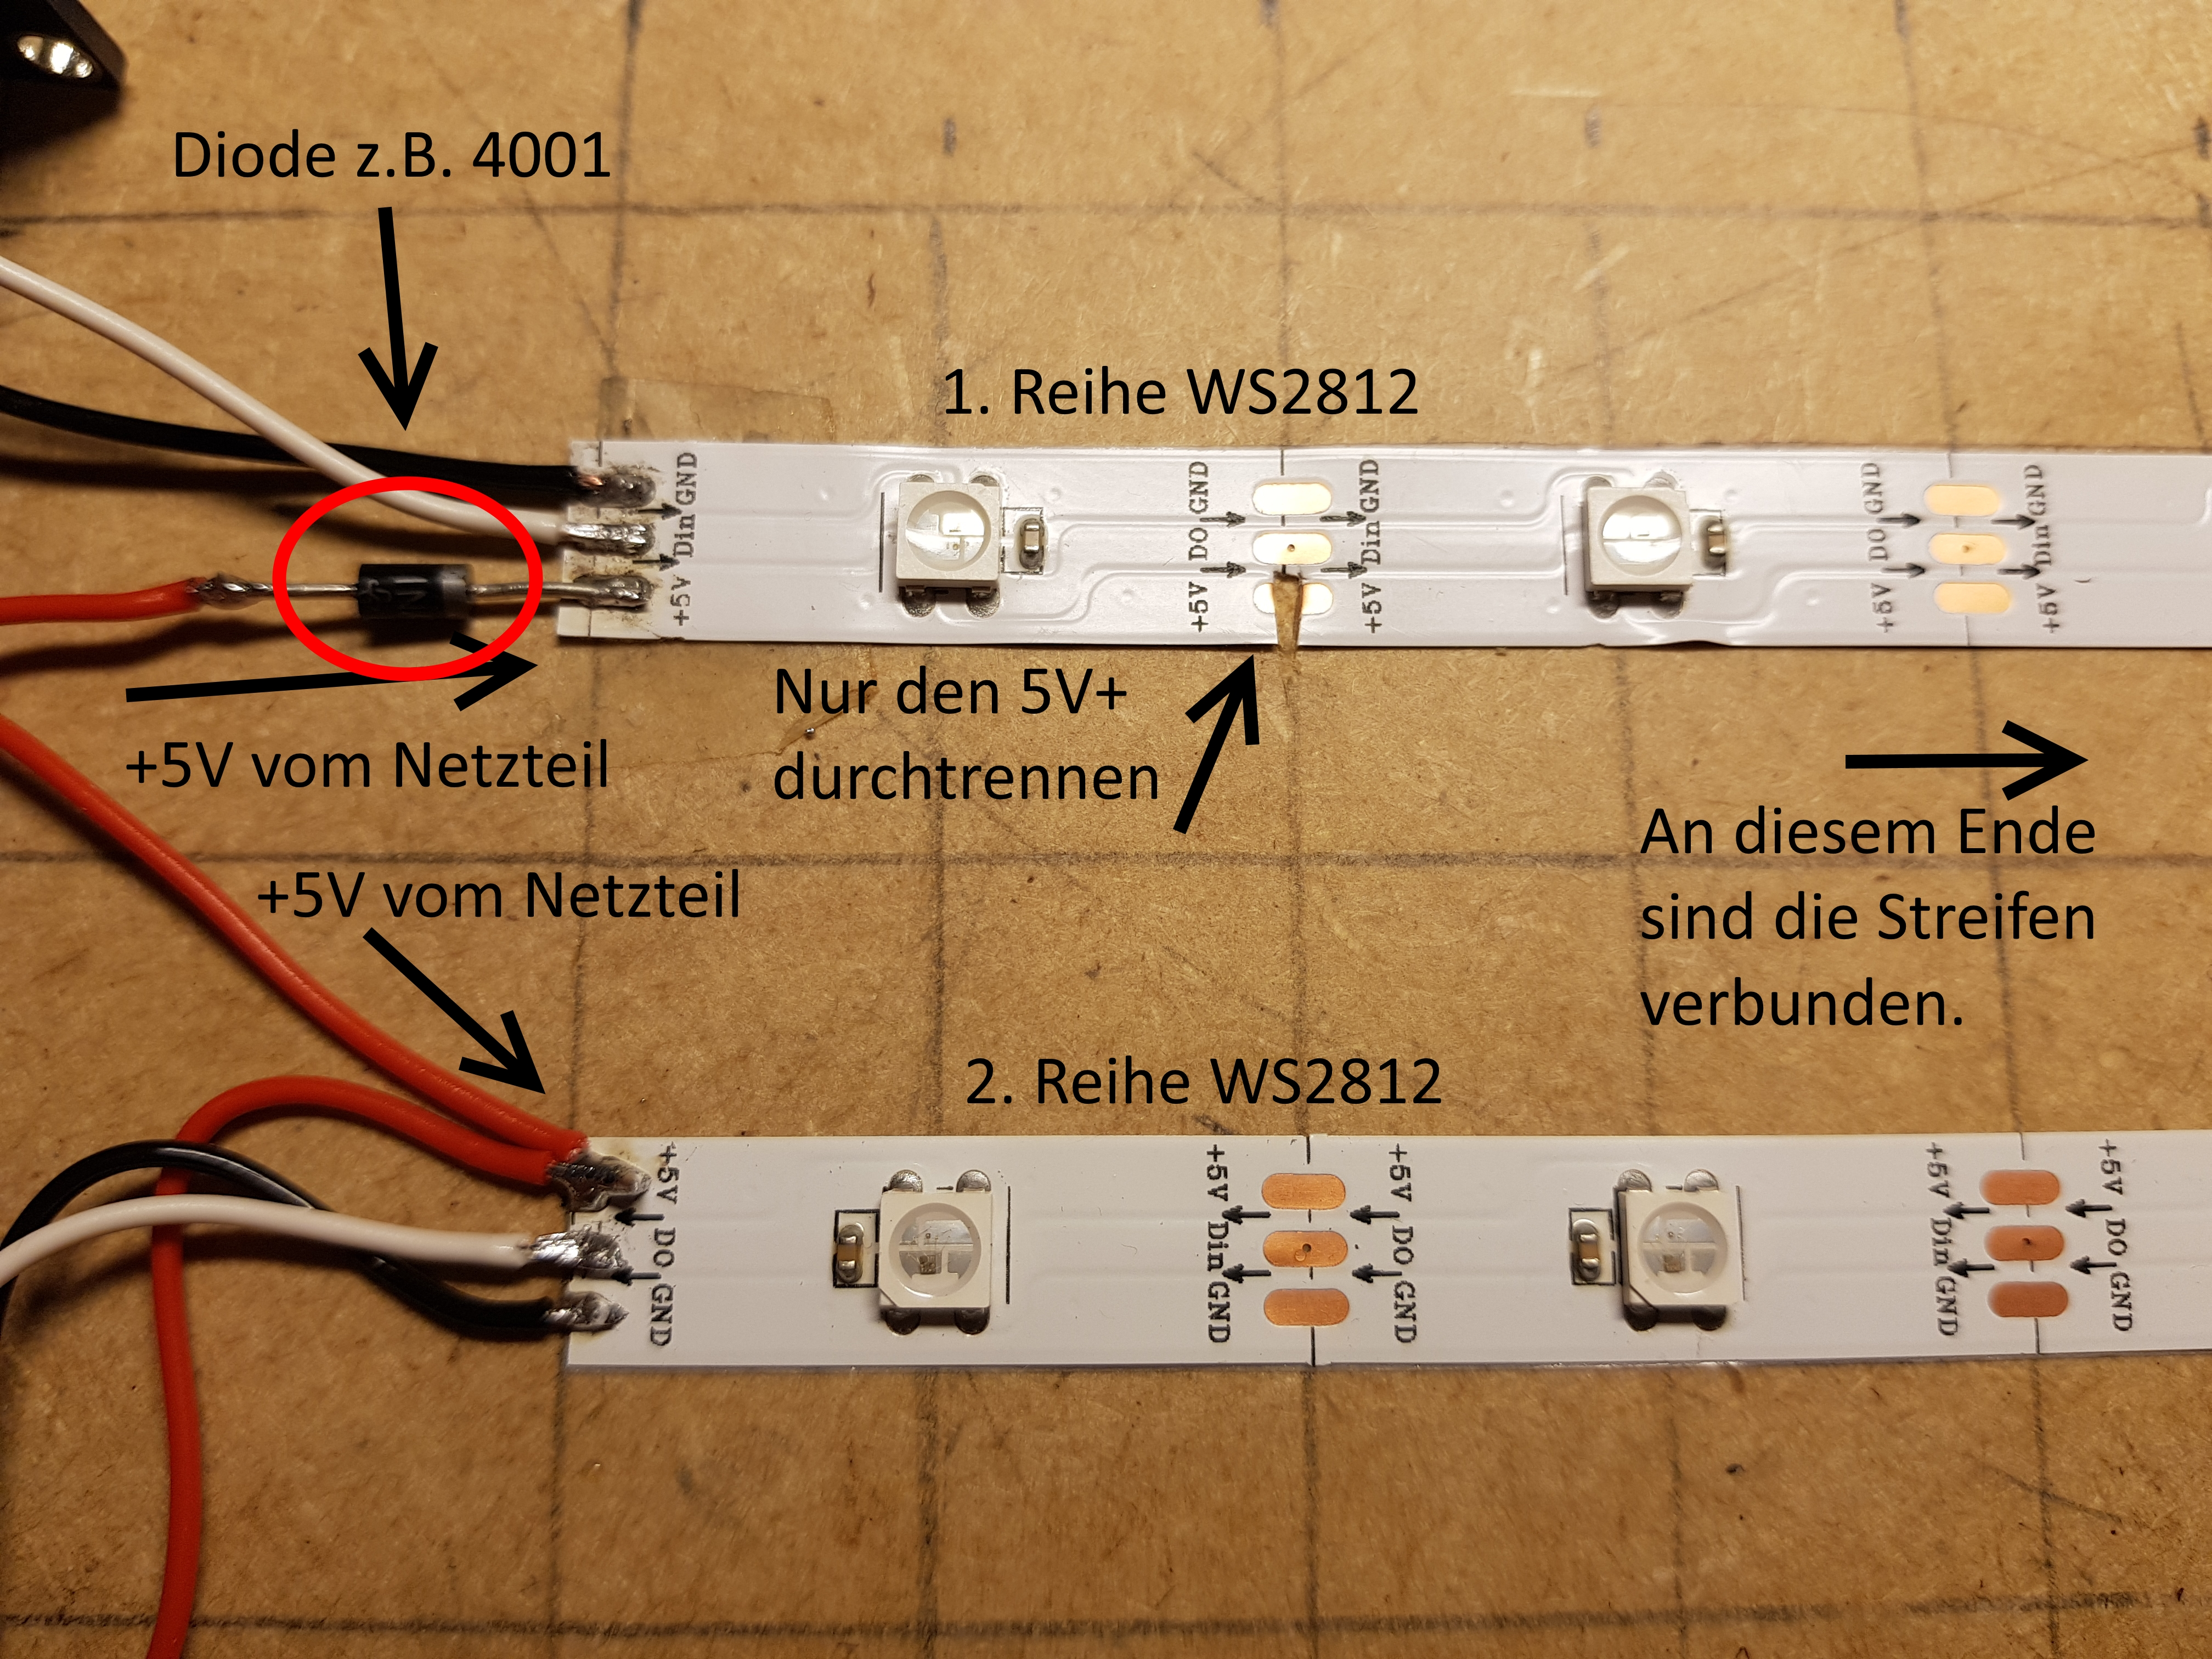
\includegraphics[width=\linewidth]{Logos/Schematic.pdf} 
		\caption{Anschlussbeispiel}
		\label{abb.Schematic}
	\end{figure}

\chapter{Funktionen der Uhrensoftware auf dem ESP}

\section{Verbinden der Uhr mit dem eigenen WLAN}
Nach dem erfolgreichen Verbinden kann die Uhr nach Eingabe der angezeigten IP-Adresse in einem Browser konfiguriert werden. Dabei kann die Uhr auch mit dem eigenen WLAN Netz verbunden werden.
 
\section{Zeitserver (NTP Server)}
Falls die Uhr an das eigene WLAN mit Internet angebunden wird, kann ein Zeitserver hinterlegt werden. Dieser sorgt dafür, dass die Uhrzeit zyklisch sekundengenau gestellt wird. 
 
\section{Automatische Helligkeitsregelung}
Falls der optionale LDR an der Uhr angeschlossen wurde, ist es möglich, die Helligkeit automatisch, abhängig der Umgebungshelligkeit, regeln zu lassen. Dazu muss folgende Einstellung aktiviert werden. Durch das Feld Kalibrierung kann man die Grundhelligkeit an seine eigenen Wünsche anpassen.

\end{document}
